\section{Introduction}

Expansion-based formulations of the Fermi paradox connect technological capability to persistent settlement or self-replicating activity. \citet{Hart1975} and \citet{Tipler1980} gave influential versions of this argument; \citet{Brin1983} reviewed the broader assumptions behind the resulting ``Great Silence.'' Diffusion, finite settlement lifetimes, stellar motion, and heterogeneous sites complicate the route from launch capability to complete occupation \citep{NewmanSagan1981,CarrollNellenback2019}. Cosmological models nevertheless show why even a small number of persistently expanding lineages can matter \citep{Olson2015,Hanson2021,Kipping2026}. This paper examines a behavioural premise rather than denying these propagation arguments: does a civilization that can expand necessarily continue to find additional external investment worthwhile?

The computational inward transition hypothesis (\CITH) considers continued growth directed inward. Virtual worlds may contain agents or processes that generate further worlds, producing an approximately self-similar hierarchy of designed environments, institutions, histories, and experiences. A civilization need not become passive or lose its ambition. It may increase the quantity, variety, or quality of valued activity without repeatedly establishing resident infrastructure elsewhere. Technological progress may also make the supporting services of a chosen internal growth path sufficiently available within existing territory. The strong hypothesis combines these possibilities: \emph{continued internal growth can coexist with no additional external investment when local support remains sufficient and the relevant allocation inequalities continue to hold.} Recursively nested worlds motivate a workload-accounting example; the allocation mechanism does not require recursion.

This is not the assertion that an ordinary finite computer implements infinitely many independent worlds at once. Nor is a computer inside a simulation an additional physical computer that can be added to the host's capacity. \CITH\ is a production and allocation hypothesis subject to physical accounting, not a source of free substrate. Energy, state storage, entropy management, replacement material, error correction, and failure risk remain relevant \citep{Landauer1961,Bennett1973,Lloyd2000}. The distinction between a generative rule and its instantiated states will be explicit.

\subsection{Relation to earlier work and the claimed contribution}

The qualitative ideas of postbiological civilizations and inward development are not new. \citet{Dick2003} and \citet{CirkovicBradbury2006} considered computationally oriented civilizations; \citet{Smart2012} proposed transcension toward increasingly dense internal scales. Aestivation concerns the timing of computation rather than substituting internal development for external investment \citep{Sandberg2017}. The thermodynamic critique by \citet{BennettHansonRiedel2019} is important here: efficiency cannot be evaluated without specifying accessible entropy reservoirs. Sustainability and homeostasis offer different mechanisms for bounded growth \citep{HaqqMisraBaum2009,WongBartlett2022}. The present paper neither imports a universal evolutionary destiny nor infers preferences from energy efficiency alone.

A non-peer-reviewed working paper uses the phrase ``Inward Transition'' for a post-AGI shift toward internal computation and reduced detectability \citep{Pitti2026}. No priority is claimed for that phrase, virtual worlds, or inwardness. Conversely, resource acquisition and self-replicating industry can strengthen expansion incentives, including on intergalactic scales \citep{ArmstrongSandberg2013}; autonomous machine industry may reduce dependence on biological settlement \citep{Ivliev2026}. Population-total value can make unused astronomical resources represent substantial foregone welfare \citep{Bostrom2003Waste}. These are direct counterpressures, not exceptions to be excluded by definition. Social-scientific critiques also caution against treating poorly identified motives or human scaling laws as universal civilizational laws \citep{Shkurko2024,JacksonCriadoPerez2024}.

The proposed contribution is a more specific combination: a workload frontier, a common-budget comparison of internal and external activity, exact logarithmic thresholds, a curvature trichotomy, and pathwise persistence conditions. Access costs, larger budgets, residual external value, production curvature, and future resource production supply explicit tests of the mechanism. The optimization and branching-process tools are standard. Their application identifies assumptions that a strong inward-growth claim must satisfy and circumstances in which it fails. The analytical thresholds, rather than a fraction of a synthetic ensemble, are the main result.

\subsection{Four distinct claims}

The strong inward-growth claim must be separated from three neighbouring statements. First, fewer new resident settlements may coexist with extensive external mining and probes; this is a weaker \emph{settlement-composition} branch. Second, either branch could be bright or faint. Third, even common inward allocation need not explain galactic silence because autonomous expansionist descendants can dominate territory. We distinguish the \emph{allocation claim}, the \emph{detectability claim}, and the \emph{population claim}. The formal focus is all-inward allocation, not merely reduced settlement. Neither detectability nor a population-level explanation of silence follows from that allocation alone.

\section{Workload accounting and local resource sufficiency}
\label{sec:support}

\subsection{Experiential substitution does not create external facts}

Let $q\in[0,1]$ represent decision-relevant experiential fidelity, with an increasing substitution map $\sigma(q)\in[0,1]$. If $E(n)$ is the experiential benefit of additional residence before substitution, and $X(n)$ is residual value, write
\begin{equation}
 B_{\rm phys}(n,q)=[1-\sigma(q)]E(n)+X(n).
 \label{eq:experiential}
\end{equation}
At perfect substitution only the first term disappears. Unknown independent histories, raw material, strategic options, or a preference for physical authenticity may remain valuable. For a discrete project with substitutable value $e_j$, residual value $x_j$, and incremental cost $c_j$ relative to an internal alternative,
\begin{equation}
 \Delta_j(q)=[1-\sigma(q)]e_j+x_j-c_j.
 \label{eq:premium}
\end{equation}
A positive reality premium is compatible with rejecting the project when it does not cover its extra cost. This is not an assertion of metaphysical identity between a simulated and an external object.

The reduced-form $q$ is domain-specific. It does not measure consciousness, establish the moral equivalence of digital minds, or imply that simulated observations reveal unknown external facts. An embodied population using virtual environments is sufficient for the weaker experiential interpretation. The recursive digital-population interpretation additionally assumes that the relevant minds can be realized computationally.

\subsection{Generative depth and implemented workload}

Consider a regular illustrative hierarchy with integer branching factor $b\geq2$ and maximum integer depth $d\geq0$. Its number of represented worlds is
\begin{equation}
 W_d=\sum_{j=0}^{d}b^j=\frac{b^{d+1}-1}{b-1}.
 \label{eq:worlds}
\end{equation}
A recursive rule can lack a prescribed terminal depth even though every actual execution has finite depth, finite state, and finite elapsed computation. Approximate self-similarity is an architectural description; no physical fractal dimension or infinite computational speed-up is inferred from it. A hierarchy need not be regular in applications, and counts alone do not measure novelty or welfare.

For a fully instantiated hierarchy, let $u_k>0$ be the normalized per-world requirement for physical service $k$, $\eta_k>0$ a stated efficiency factor, and $K_k$ the locally available capacity in matching units. Examples of $k$ include update work during an interval, persistent memory, heat rejection, and material replacement. The simplifying homogeneous accounting is
\begin{equation}
 D_k(d)=\frac{u_kW_d}{\eta_k},\qquad D_k(d)\leq K_k\quad\text{for every }k.
 \label{eq:resource}
\end{equation}
These are separate constraints, not quantities to be added without a common conversion. For cumulative energy or material consumption, $D_k$ and $K_k$ must refer to integrated demand and the available stock over the same horizon. Instantaneous power cannot be compared with lifetime energy.

\begin{lemma}[Finite-depth support frontier]
\label{prop:depth}
Under \cref{eq:resource}, define $Q=\min_k K_k\eta_k/u_k$. If $Q\geq1$, the largest feasible integer depth is
\begin{equation}
 d_{\max}=\left\lfloor\log_b[1+(b-1)Q]-1\right\rfloor.
 \label{eq:depth-bound}
\end{equation}
If $Q<1$, even the root world at the specified workload is infeasible. Finite positive $K_k\eta_k/u_k$ for at least one service imposes a finite depth ceiling.
\end{lemma}
\begin{proof}
Every service constraint is equivalent to $W_d\leq K_k\eta_k/u_k$. Their intersection is $W_d\leq Q$. Substitution of \cref{eq:worlds}, followed by taking a logarithm and restricting $d$ to integers, gives \cref{eq:depth-bound}.
\end{proof}

The lemma does not forbid continued creation of worlds. It specifies the trade-off. Deeper simultaneous hierarchies require more effective support, less per-world workload, or a different execution schedule. The $u_k$ parameters include whatever fidelity, update rate, individuality, addressing, and coordination the stipulated worlds require. Compression is not assumed to remove independent state information without loss.

A scheduled hierarchy requires a different account. Processing and heat may depend on the active set $A(t)\leq W_{d(t)}$, but preserved inactive states still consume memory. Reusing a program description does not remove accumulated histories. The numerical example below therefore charges processing and heat to the active worlds and persistent memory to \emph{all} represented world states. Scheduling changes simultaneity and completion time; it is not a demonstration that arbitrary independent worlds can all be lived at full speed with constant resources.


\paragraph{What recursion adds.}
For the fully instantiated hierarchy at fixed per-world workload and efficiency, \cref{eq:worlds} gives
$W_{d+1}=bW_d+1$, and hence
\begin{equation}
 \frac{D_k(d+1)}{D_k(d)}=b+\frac{1}{W_d}\longrightarrow b.
 \label{eq:recursion-cost}
\end{equation}
If useful computation is proportional to fully instantiated workload,
$C_d=cW_d$ with fixed $c>0$, logarithmic value adds only
\begin{equation}
 F(C_{d+1})-F(C_d)
 =\ln\!\left[\frac{1+c(bW_d+1)}{1+cW_d}\right]
 \longrightarrow\ln b.
 \label{eq:recursion-value}
\end{equation}
Both limits follow by dividing numerator and denominator by $W_d$ and
using $W_d\to\infty$. Thus deeper nesting is not a computational free
lunch. Recursion supplies a concrete generative workload, not a distinct
preference mechanism: replacing it by any non-recursive internal workload
with the same service demands and computational value leaves the allocation
results in sections~3--5 unchanged.

\subsection{Support over a development path}

For a specified horizon $[0,T]$, local sufficiency means
\begin{equation}
 \chi_T=\sup_{0\leq t\leq T}\max_k\frac{D_k(t)}{K_k(t)}\leq1.
 \label{eq:chi}
\end{equation}
Reliability also requires an explicit service criterion; extra local copies need not remove common-mode failures. Technological progress can reduce $u_k$, increase usable $\eta_k$ or $K_k$, improve repair, or alter the execution schedule. These are possible pathways, not measured capabilities. In particular, reversible computation does not authorize neglecting state preparation, error management, or the entropy reservoirs actually available \citep{Bennett1973,BennettHansonRiedel2019}.

A simple rate comparison clarifies the temporal issue. If a service ratio evolves as $\chi_k(t)=\chi_{k0}\exp[(g_{D,k}-g_{K,k})t]$, it crosses one at
\begin{equation}
 T_k=\frac{\ln(1/\chi_{k0})}{g_{D,k}-g_{K,k}}
 \label{eq:crossing}
\end{equation}
when $0<\chi_{k0}<1$ and demand growth exceeds capacity growth. A finite-horizon success does not imply sufficiency at every future time. Conversely, external acquisition is not required by this accounting over an interval on which all demands are met locally.

Four controlled examples use $b=2$, $d(t)=2+\lfloor t/10\rfloor$ on $0\leq t\leq40$, and local capacities $(32,256,24)$ for update work, stored-state memory, and heat rejection. All $u_k=1$. Processing and thermal efficiency either grow as $e^{0.12t}$, grow as $e^{0.01t}$, or grow as $e^{0.12t}$ up to a ceiling of four; memory efficiency remains one. A fourth example activates at most eight worlds at a time without efficiency improvement. Every example stores all $W_d$ states. These are normalized accounting constructions, not device specifications.

The matched-efficiency example remains feasible while the full hierarchy grows from seven to 127 worlds. Demand outpacing efficiency first violates a constraint at $t=20$, and the efficiency-ceiling example first violates one at $t=40$. Scheduling remains feasible on the tested interval, but only eight worlds are active at once. The maximum ratios are respectively $0.4961$, $3.5471$, $1.3229$, and $0.4961$. All changes in depth occur at known times, so interval maxima can be checked at the jumps rather than inferred from a sampled time grid alone. \Cref{fig:support} illustrates the distinction between technology-supported expansion of internal activity and merely postponing a resource limit. Extending the matched-efficiency path with the same fixed memory efficiency and capacity gives $W=255$ and a memory ratio $255/256=0.99609375$ at $t=50$, but $W=511$ and $511/256=1.99609375$ at $t=60$. The latter is its first memory violation. The example therefore supports the stated finite horizon, not indefinite local sufficiency.

\begin{figure}[tbp]
\centering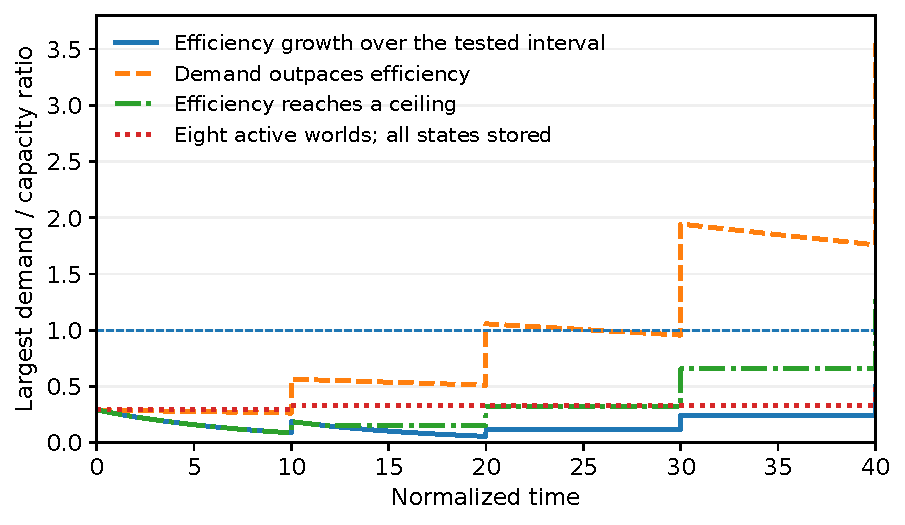
\includegraphics[width=.95\textwidth]{fig1.pdf}
\caption{Finite-horizon local support constructions. The largest service-demand ratio must remain at or below one. Processing and heat are charged to active worlds; persistent memory is charged to all represented states, including inactive ones. Growth in depth is stepwise. No curve is extrapolated to unlimited time, and no physical implementation is validated.}
\label{fig:support}
\end{figure}

\section{Allocation between inward growth and external projects}
\label{sec:allocation}

Feasibility and optimality are different questions. Even a locally supportable civilization may prefer to acquire further resources. To test that preference without removing the internal alternative, let $z,x,y,w\geq0$ denote intensive local investment, additional resident infrastructure, industry-only capacity, and observation-only capacity. With local investment as numeraire, the common budget is
\begin{equation}
 z+p_nx+p_hy+p_mw\leq B,\qquad p_j>0,\quad B>0.
 \label{eq:budget}
\end{equation}
All quantities are normalized within one planning horizon. The cumulative indices $n=1+x$, $h=1+x+y$, and $m=1+x+y+w$ distinguish residence, industry, and observation. They are continuous service-capacity indices in this model, not literal fractional star systems. The nesting is an accounting assumption, not a necessary geometry of every civilization. Their use does not assume that star systems themselves are divisible.

Consider
\begin{align}
 C&=C_0+a\ln(1+z)+r_nx+r_hy,\label{eq:compute}\\
 U&=F(C)+(1-q)E(x)+\epsilon_RR(x+y)+\epsilon_II(x+y+w),\label{eq:utility}
\end{align}
where $a>0$, $C_0\geq0$, $r_n,r_h\geq0$, and the residual weights are non-negative. The specialization $\sigma(q)=q$ is used here. $C$ is useful computational service over the horizon, not a count of simulated hardware added to real hardware. $E$ is substitutable settlement-specific experience; $R$ and $I$ represent residual resilience and independent-information value. The common budget prevents counting external investment as beneficial without comparing what the same resources could produce internally.

A small $\epsilon_R$ or $\epsilon_I$ means low residual marginal value in the objective. Hard energy, reliability, or material requirements are separate feasibility constraints, as in \cref{eq:chi}; the sensitivity scenarios therefore use the label \emph{large residual values}.

\subsection{An all-inward optimum without bounded total value}

Assume $F$ is differentiable, strictly increasing, and concave, and $E,R,I$ are differentiable, non-decreasing, and concave on the feasible domain. Composition with the concave $C$ makes $U$ concave. Positive $a$ and increasing $F$ exhaust the budget. At the all-inward corner $(z,x,y,w)=(B,0,0,0)$ define
\begin{align}
 C_L&=C_0+a\ln(1+B),&
 \lambda_L&=F'(C_L)\frac{a}{1+B},\label{eq:local-return}\\
 D_n&=F'(C_L)r_n+(1-q)E'(0)+\epsilon_RR'(0)+\epsilon_II'(0),\nonumber\\
 D_h&=F'(C_L)r_h+\epsilon_RR'(0)+\epsilon_II'(0),&
 D_m&=\epsilon_II'(0).\label{eq:external-return}
\end{align}

\begin{proposition}[All-inward allocation]
\label{prop:corner}
For \cref{eq:budget,eq:utility} under the stated differentiability and concavity assumptions, the all-inward corner is globally optimal if and only if
\begin{equation}
 \frac{D_j}{p_j}\leq\lambda_L\qquad(j=n,h,m).
 \label{eq:corner}
\end{equation}
If all three inequalities are strict, every optimizer has zero external investment. Equality can admit ties; uniqueness is not asserted from a weak inequality.
\end{proposition}
\begin{proof}
For any feasible displacement from the corner, the supporting-hyperplane inequality gives
\begin{align}
 U(z,x,y,w)-U(B,0,0,0)
 &\leq\lambda_L(z-B)+D_nx+D_hy+D_mw\nonumber\\
 &\leq(D_n-p_n\lambda_L)x+(D_h-p_h\lambda_L)y
 +(D_m-p_m\lambda_L)w.
 \label{eq:cornerproof}
\end{align}
The right side is non-positive under \cref{eq:corner}, and strictly negative for any positive external component if all inequalities are strict. Conversely, transferring a sufficiently small budget amount from $z$ to a violating external direction has positive directional derivative and improves the objective.
\end{proof}

This is the standard supporting-hyperplane or first-order optimality criterion for a concave maximization problem \citep[chapters 3--5]{BoydVandenberghe2004}, specialized to the civilizational allocation model. It does not require bounded total ambition: $F(C)=\ln(1+C)$ grows without bound as $C\to\infty$. It does require specified alternatives, prices, residual preferences, and an admissible local path. Its contribution is not a new general optimization theorem, but the identification of the competing terms relevant to the hypothesis.

\begin{corollary}[Adding hard support constraints]
\label{cor:feasibility}
Suppose an additional physical feasibility restriction retains the all-inward corner. If \cref{eq:corner} holds, the corner remains optimal in the restricted problem. The inequalities need not remain necessary: at a binding physical constraint, a formerly improving external direction may no longer be feasible. Necessity is recovered when each small budget-transfer direction used in the converse proof remains admissible.
\end{corollary}
\begin{proof}
A maximum over the larger feasible set is a maximum over any subset that contains it. The converse uses only the feasibility of the indicated local directions.
\end{proof}

The corollary prevents a numerical preference calculation from being mistaken for engineering validation. An all-inward optimum with $\chi_T>1$ is not an implementable explanation of the chosen workload. An outward optimum despite $\chi_T\leq1$ describes attractive expansion, not expansion forced by a local shortfall. The two tests must be reported separately.

\subsection{Exact thresholds and computational-value curvature}
\label{sec:threshold}

Specialize to $F(C)=\ln(1+C)$. Write the residual slopes as
\begin{align}
 S_n&=(1-q)E'(0)+\epsilon_RR'(0)+\epsilon_II'(0),\nonumber\\
 S_h&=\epsilon_RR'(0)+\epsilon_II'(0),& S_m&=\epsilon_II'(0),
 \label{eq:slopes}
\end{align}
and set $r_m=0$, $L=\ln(1+B)$ and $d_0=1+C_0$. Define
\begin{equation}
 H_j=(1+B)L S_j,\qquad A_j=(1+B)(r_j+d_0S_j).
 \label{eq:HA}
\end{equation}
Direct substitution into \cref{eq:corner} gives the exact equivalent test
\begin{equation}
 \boxed{p_j\geq H_j+\frac{A_j}{a}\quad\text{for all }j.}
 \label{eq:exact}
\end{equation}
No numerical optimizer is needed to determine whether this corner is optimal.

\begin{proposition}[Productivity threshold and residual floor]
\label{prop:threshold}
Hold $B,C_0,p_j,r_j,S_j$ fixed. Assume at least one $A_j>0$; if none is positive every $a>0$ is inward. For every direction with $A_j>0$, a finite productivity level satisfying \cref{eq:exact} exists if and only if $p_j>H_j$. When all relevant denominators are positive,
\begin{equation}
 a\geq a_{\rm crit}:=\max_{j:A_j>0}\frac{A_j}{p_j-H_j}
 \label{eq:acrit}
\end{equation}
is necessary and sufficient. A direction with $A_j=0$ imposes no restriction because then $r_j=S_j=H_j=0$. If any $A_j>0$ has $p_j\leq H_j$, no finite increase of $a$ alone produces an all-inward corner.
\end{proposition}
\begin{proof}
All factors used to obtain \cref{eq:exact} are positive. Rearranging $A_j/a\leq p_j-H_j$ yields the result; the zero case follows from non-negativity of its constituent terms.
\end{proof}

The quantity $H_j$ is a \emph{residual-value floor relative to local marginal return}, not an irreducible energy cost or a physical impossibility theorem. It shows precisely why ``better computers'' alone can fail: external information or other residual value may remain competitive even when remote computational value becomes relatively small. Improving substitution or local support can alter these residual preferences, but their disappearance must not be silently assumed.

A dimensionless robustness diagnostic is
\begin{equation}
 \rho=\max_j\frac{H_j+A_j/a}{p_j}.
 \label{eq:rho}
\end{equation}
The corner is inward when $\rho\leq1$. If every external price is multiplied by $\kappa>0$ while other terms are held fixed, the corner survives exactly when $\kappa\geq\rho$. Thus reporting $\rho$ identifies how much a conclusion depends on proximity to a threshold. This is conditional price sensitivity, not a distribution over unknown technologies.

\paragraph{Curvature generalization.}

Use the normalized shifted-isoelastic family
\begin{equation}
 F_\eta(C)=
 \begin{cases}
 \big[(1+C)^{1-\eta}-1\big]/(1-\eta),&\eta\neq1,\\
 \ln(1+C),&\eta=1,
 \end{cases}
 \qquad \eta\geq0.
 \label{eq:isoelastic}
\end{equation}
Thus $F_\eta'(C)=(1+C)^{-\eta}$, $F_\eta(0)=0$ and
$F_\eta'(0)=1$. The restriction $\eta\geq0$ retains concavity;
negative $\eta$ is outside the global corner theorem. The curvature
parameter $\eta$ is distinct from the service-efficiency factors $\eta_k$.

\begin{proposition}[Curvature trichotomy for inward allocation]
\label{prop:curvature}
Fix $B>0$, $d_0\geq1$, $p_j>0$ and finite $r_j,S_j\geq0$, and set
$L=\ln(1+B)$. Under the common-budget model and its concavity
assumptions, a direction satisfies the all-inward test exactly when
\begin{equation}
 r_j+S_j(d_0+aL)^\eta\leq\frac{p_j a}{1+B}.
 \label{eq:iso-corner}
\end{equation}
For $0\leq\eta<1$, every nontrivial direction has a unique finite
threshold, and the all-inward corner is optimal for every $a$ above the
largest of those thresholds. For $\eta=1$, the exact condition is
$p_j\geq H_j+A_j/a$; a finite threshold exists if and only if
$p_j>H_j$ in every nontrivial direction. For $\eta>1$, the inward set
in $a>0$ for each direction with $S_j>0$ is either empty, a singleton,
or a bounded closed interval. Consequently, if any direction has
$S_j>0$, sufficiently high productivity precludes an all-inward corner.
Directions with $S_j=0$ retain the threshold
$a\geq(1+B)r_j/p_j$ for every $\eta$; a direction with $r_j=S_j=0$
is unrestricted.
\end{proposition}
\begin{proof}
At the corner, $1+C_L=d_0+aL$. The local marginal return is
$a/[(1+B)(d_0+aL)^\eta]$, and direction $j$ has marginal return
$r_j/(d_0+aL)^\eta+S_j$. The first-order condition from
Proposition~\ref{prop:corner}, multiplied by the positive quantity
$(d_0+aL)^\eta$, gives \eqref{eq:iso-corner}. Since $F_\eta$ is
increasing and concave for $\eta\geq0$, that condition remains necessary
and sufficient for global optimality when it holds in all directions.

For a nontrivial direction define its required relative price
\[
 P_{j,\eta}(a)=\frac{1+B}{a}\big[r_j+S_j(d_0+aL)^\eta\big].
\]
For $0\leq\eta<1$, differentiation gives
\[
 P_{j,\eta}'(a)=\frac{1+B}{a^2}
 \left\{-r_j+S_j(d_0+aL)^{\eta-1}
 \big[(\eta-1)aL-d_0\big]\right\}<0.
\]
The strict inequality follows from nontriviality, $d_0>0$ and
$\eta<1$. Moreover, $P_{j,\eta}(a)\to\infty$ as $a\downarrow0$,
whereas $P_{j,\eta}(a)\to0$ as $a\to\infty$: its two terms are of
orders $a^{-1}$ and $a^{\eta-1}$, respectively. Continuity and strict
monotonicity imply exactly one solution of $P_{j,\eta}(a)=p_j$,
and the direction passes precisely above it. Taking the maximum over
finitely many directions proves the first case. At $\eta=1$, expansion
of the bracket gives $P_{j,1}(a)=H_j+A_j/a$, proving the second case,
including the strictly positive denominator requirement.

For $\eta>1$ and $S_j>0$, put
\[
 D_j(a)=r_j+S_j(d_0+aL)^\eta-\frac{p_j a}{1+B}.
\]
Then $D_j(0)=r_j+S_jd_0^\eta>0$ and
\[
 D_j''(a)=S_j\eta(\eta-1)L^2(d_0+aL)^{\eta-2}>0.
\]
Also $D_j(a)\to\infty$ as $a\to\infty$, because its positive
$a^\eta$ term dominates its linear term. Its non-positive sublevel set
is convex by convexity, closed by continuity, bounded by this divergence,
and bounded away from zero by $D_j(0)>0$. It is therefore empty, a
singleton, or a bounded closed interval contained in $(0,\infty)$.
The intersection over directions is bounded if any such direction exists.
Finally, with $S_j=0$, \eqref{eq:iso-corner} reduces directly to the
stated threshold, including the unrestricted zero-return case.
\end{proof}
The finite, positive high-productivity price limit is specific to
$\eta=1$: it is zero for $\eta<1$, equals $H_j$ for $\eta=1$, and
diverges for $\eta>1$ when $S_j>0$. Thus it would be incorrect to say
that only logarithmic value allows residual benefits to defeat increases
in productivity. The distinction is between a finite asymptotic floor and
an unbounded high-productivity requirement. The $\eta>1$ branch has
bounded total computational value; the $0\leq\eta\leq1$ branches do not.

For the normalized example $B=10$, $r=0.1$, $S=0.001$, $d_0=2$,
$p=1$ and $\eta=2$, \eqref{eq:iso-corner} is a quadratic inequality.
The quadratic roots are $a_-\simeq1.421897$ and $a_+\simeq12.720521$, with inward
allocation exactly on $[a_-,a_+]$. Separate scalar maximizations of a
concave objective with residual utility $S(1-e^{-x})$ verify inward
solutions at $a=2$ and $a=10$, and outward solutions at $a=1$ and $a=20$.

\subsection{A joint finite-interval witness}

The support and allocation examples need not be merely disconnected illustrations. Couple the matched-efficiency schedule in \cref{sec:support} to $B=10$, $C_0=0$, $a(t)=W_{d(t)}/\ln(11)$, $r_n=r_h=0.1$, and all three prices equal to one. Set $q=0.99$, $\epsilon_R=\epsilon_I=0.001$, with unit initial slopes for $E,R,I$. At $z=B$, useful computation is exactly $C_L=W_{d(t)}$, the workload charged in the support example. The three outward-to-local marginal-return ratios are
\begin{equation}
 11\ln(11)\left[S_j+\frac{r_j+S_j}{W_{d(t)}}\right],
 \qquad(S_n,S_h,S_m)=(0.012,0.002,0.001).
 \label{eq:joint-witness}
\end{equation}
They decrease with world count and are already below one at seven worlds. Thus this same finite family satisfies both the three-service feasibility test and strict all-inward optimality with positive residual external values. As the hierarchy grows from seven to 127 worlds, attained logarithmic value rises from $\ln8$ to $\ln128$. The budget is fixed at $B=10$ and productivity is deliberately tuned to $a(t)=W_{d(t)}/\ln 11$. This is a consistency witness, not evidence for the plausibility of that productivity path, an engineering implementation, or an infinite-horizon optimum. Persistent memory is still charged to every world; future resource effects are considered separately in \cref{sec:dynamic}.

\subsection{Budget growth and shared technological progress}

With perfect experiential substitution and no residual external value, $q=1$ and $\epsilon_R=\epsilon_I=0$. For \emph{any} strictly increasing $F$, maximizing value is equivalent to maximizing $C$. Let
\begin{equation}
 R_* = \max\{r_n/p_n,r_h/p_h\}.
 \label{eq:Rstar}
\end{equation}
When $R_*>0$, the solution allocates
\begin{equation}
 z^*=\min\{B,\max(a/R_*-1,0)\},\qquad
 B_{\rm crit}=a/R_*-1.
 \label{eq:budgetcrit}
\end{equation}
Any remaining budget goes to a best-return computational external channel. The all-inward condition is $a/(1+B)\geq R_*$. If $R_*=0$, all investment is local. This exposes a limitation of a fixed-budget productivity path: with fixed $a$ and $R_*>0$, a sufficiently large budget restores external investment even without authenticity, information, or resilience premiums. The civilization does not stop preferring more value when it can generate virtual worlds.

If local and remote computational coefficients all receive the same multiplicative improvement, the pure-computation condition is unchanged. Progress that disproportionately raises intensive return can support inward allocation; progress that improves everything equally need not. \Cref{fig:budget} shows this budget effect for $R_*=1$. Persistent inward allocation along a development path requires the relevant inequalities to hold along that path, not merely at one chosen value of $B$.

\begin{figure}[tbp]
\centering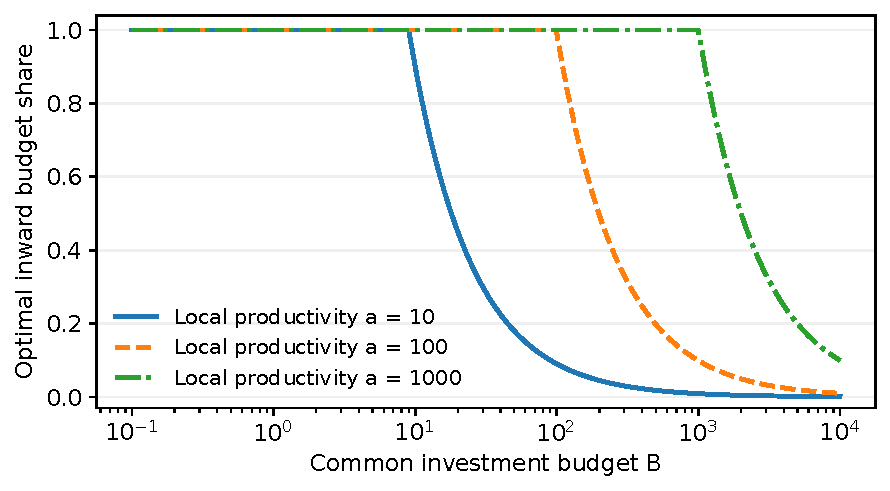
\includegraphics[width=.95\textwidth]{fig2.pdf}
\caption{Exact inward budget share with perfect experiential substitution, zero residual value, and $R_*=1$. The transition occurs at $B=a-1$. Greater local productivity moves the boundary, but budget growth can eventually favor additional external capacity. Any strictly increasing computational value function gives the same allocation in this pure-computation case.}
\label{fig:budget}
\end{figure}

\paragraph{Persistence when budgets grow.}

For logarithmic computational value, let $d_0=1+C_0\geq1$ and
$r_j\geq0$ be fixed. At time $t$, define
\[
 L(t)=\ln[1+B(t)],\qquad
 H_j(t)=[1+B(t)]L(t)S_j(t),\qquad
 A_j(t)=[1+B(t)][r_j+d_0S_j(t)].
\]
All quantities below are finite at each finite time. Prices are relative to
local investment, the numeraire.

\begin{proposition}[Pathwise persistence with logarithmic value]
\label{prop:persistence}
Suppose $B(t)>0$, $a(t)>0$, $p_j(t)>0$ and $S_j(t)\geq0$ on a
path $t\geq t_0$, and retain the differentiability and concavity assumptions
of Proposition~\ref{prop:corner}. The all-inward corner is optimal at every
time on this path if and only if, for every $t$ and every direction with
$A_j(t)>0$,
\begin{equation}
 p_j(t)>H_j(t),\qquad
 a(t)\geq \max_{j:A_j(t)>0}
 \frac{A_j(t)}{p_j(t)-H_j(t)}.
 \label{eq:pathwise}
\end{equation}
The maximum over an empty set is zero. In particular, wherever $S_j(t)>0$,
\begin{equation}
 \frac{p_j(t)}{S_j(t)}>[1+B(t)]\ln[1+B(t)].
 \label{eq:path-ratio}
\end{equation}
If $B(t)\to\infty$, a bounded price and a residual slope bounded away
from zero in even one direction preclude eventual all-inward allocation,
regardless of $a(t)$. With a fixed positive residual slope, persistence
requires its relative external price to grow at least on the order of
$B(t)\ln B(t)$. With bounded prices, it instead requires
$S_j(t)=O(1/[B(t)\ln B(t)])$ for each direction. These order conditions
are necessary, not sufficient: the productivity inequality in
\eqref{eq:pathwise} must also hold. If $S_j(t)=0$ but $r_j>0$, that
inequality reduces to $a(t)\geq[1+B(t)]r_j/p_j(t)$.
\end{proposition}
\begin{proof}
At each time, the exact logarithmic corner test is
$p_j(t)\geq H_j(t)+A_j(t)/a(t)$. If $A_j(t)>0$ and $a(t)$ is
finite and positive, this requires $p_j(t)>H_j(t)$; rearrangement gives
the stated lower bound on $a(t)$. Conversely these two inequalities imply
the exact test. If $A_j(t)=0$, non-negativity and $d_0>0$ imply
$r_j=S_j(t)=H_j(t)=0$, so that direction imposes no restriction.
This proves the pointwise equivalence and therefore the pathwise one.
For $S_j(t)>0$, we have $A_j(t)>0$, and division of $p_j(t)>H_j(t)$
by $S_j(t)$ gives \eqref{eq:path-ratio}. Set
$G(B)=(1+B)\ln(1+B)$. Then $G(B)\to\infty$ and
$G(B)/(B\ln B)\to1$ as $B\to\infty$. If $p_j(t)\leq M$ and
$S_j(t)\geq s>0$ eventually, $H_j(t)\geq sG(B(t))>M$ eventually,
contradicting \eqref{eq:pathwise}. The same ratio inequality gives
$p_j(t)>S_jG(B(t))$ when the slope is fixed, and
$S_j(t)<M/G(B(t))$ when prices are bounded, including any zero-slope
times. Finally, setting $S_j(t)=0$ in the exact corner test gives the
last assertion.
\end{proof}
Proposition~\ref{prop:persistence} characterizes a sequence of static
optima. In general, its conditions are neither necessary nor sufficient
for an all-inward infinite-horizon optimal policy. The two-period examples in
section~\ref{sec:dynamic} demonstrate the failure of both implications
already when only one continuation period is added.
With additional hard support constraints, necessity requires the small
budget-transfer directions used in Proposition~\ref{prop:corner} to remain
feasible; sufficiency is inherited whenever the corner remains feasible.


\subsection{Production asymmetry and concave external alternatives}
\label{sec:production}
The local term $a\ln(1+z)$ describes intensive improvement of an existing
substrate with diminishing marginal returns. Linear external terms describe
replication into additional territory over the investment range being
modelled. This intensive--extensive distinction is a modelling choice,
not a universal technological law. In particular, the unbounded logarithm
is not a physical finite-capacity constraint; such constraints are imposed
separately by the service frontier. External projects may also have
diminishing returns.

\begin{lemma}[Production curvature and the corner test]
\label{lem:production}
Replace useful computation by
\[
 C=C_0+a\ell(z)+G_n(x)+G_h(y),
\]
where $\ell$ is differentiable, increasing and concave with $\ell(0)=0$
and $\ell'(B)>0$, and $G_n,G_h$ are differentiable, non-decreasing and
concave with $G_j(0)=0$, $G_j'(0)=r_j$. Retain the original residual
utilities, set $r_m=0$, and let $F(C)=\ln(1+C)$. The all-inward corner
is globally optimal if and only if
\begin{equation}
 p_j\geq\frac{r_j+d_0S_j}{a\ell'(B)}
            +S_j\frac{\ell(B)}{\ell'(B)}
 \qquad(j=n,h,m).
 \label{eq:general-production}
\end{equation}
For $\ell(z)=\ln(1+z)$ this is exactly the original logarithmic
threshold, regardless of the curvature of $G_n,G_h$ away from zero.
\end{lemma}
\begin{proof}
The modified $C$ is concave, and composition with the increasing concave
logarithm preserves concavity of the full objective. At the corner,
$1+C_L=d_0+a\ell(B)$, the local marginal return is
$a\ell'(B)/(d_0+a\ell(B))$, and the external marginal return in
direction $j$ is $r_j/(d_0+a\ell(B))+S_j$.
The supporting-hyperplane argument of \cref{prop:corner} applies unchanged.
Multiplying its marginal-return inequality by the positive factor
$(d_0+a\ell(B))/(a\ell'(B))$ gives
\[
 p_j\geq\frac{r_j+S_j[d_0+a\ell(B)]}{a\ell'(B)},
\]
which is \cref{eq:general-production}. For the local logarithm,
$\ell(B)/\ell'(B)=(1+B)\ln(1+B)$ and
$1/\ell'(B)=1+B$, giving the stated specialization.
\end{proof}

\begin{productioncorollary}[A production-independent lower bound on the residual floor]
\label{cor:production-growth}
Retain the value, external-production and residual-utility assumptions of
Lemma~\ref{lem:production}. Let $\ell$ be increasing and concave on
$[0,\infty)$, with $\ell(0)=0$, and differentiable at the positive
corner budget $B$, where $\ell'(B)>0$. Differentiability at zero is
not required. Then the residual floor satisfies
\[
 H_j^{\ell}(B):=S_j\frac{\ell(B)}{\ell'(B)}\geq S_jB.
\]
For $S_j>0$ and finite $a>0$, an all-inward optimum requires
$p_j>H_j^{\ell}(B)\geq S_jB$. Consequently, along a path
$B(t)\to\infty$, a bounded relative external price and a residual slope
bounded away from zero in any direction exclude eventual all-inward
static allocation, regardless of productivity. A fixed positive slope
requires its relative price to grow at least linearly in $B(t)$;
bounded prices require $S_j(t)=O(1/B(t))$. These are necessary,
not sufficient, growth conditions. The faster $B\ln B$ floor for local
logarithmic production is a particular case, not a general rate.
\end{productioncorollary}
\begin{proof}
The supporting-line inequality for the concave function $\ell$, applied
at $B$ and evaluated at zero, gives
\[
 0=\ell(0)\leq\ell(B)+\ell'(B)(0-B).
\]
Since $\ell'(B)>0$, division and multiplication by $S_j\geq0$ give
$H_j^{\ell}(B)\geq S_jB$. The proof of Lemma~\ref{lem:production} needs
local differentiability only at $z=B$: the objective is concave on the
whole feasible set, and its derivatives in the feasible directions from
the inward corner exist there. Thus \cref{eq:general-production} also
holds under the present endpoint regularity. When $S_j>0$, its term
$(r_j+d_0S_j)/(a\ell'(B))$ is strictly positive, because $d_0>0$,
$r_j\geq0$ and $a$ is finite and positive. This proves
$p_j>H_j^{\ell}(B)\geq S_jB$.

If eventually $p_j(t)\leq M$ and $S_j(t)\geq s>0$, then
$S_j(t)B(t)>M$ eventually, contradicting the necessary inequality.
For fixed $S_j>0$, the same inequality gives $p_j(t)>S_jB(t)$.
For bounded prices it gives $S_j(t)<M/B(t)$ wherever $S_j(t)>0$,
with the bound immediate at zero-slope times. Neither consequence
controls the remaining productivity term in
\cref{eq:general-production}, so it does not establish sufficiency.
For $\ell(B)=\ln(1+B)$, direct substitution gives
$\ell(B)/\ell'(B)=(1+B)\ln(1+B)$, recovering the logarithmic rate.
\end{proof}

For example, $G_j(u)=r_j\ln(1+\kappa_j u)/\kappa_j$ with
$\kappa_j>0$ is concave and has the same initial slope as $r_ju$.
It preserves both the logarithmic corner test and the growth-path
obstruction in \cref{prop:persistence}. The isoelastic corner test likewise
uses only $G_j'(0)$, so \cref{prop:curvature} is unchanged. Linearity is
instead needed for the specific mixed-allocation formula in
\cref{eq:budgetcrit}, the corresponding curves in \cref{fig:budget},
and the closed-form continuation allocation in section~5.

A one-channel pure-computation example makes the distinction explicit.
Set $a=10$, $r=p=1$. With $G(x)=x$, the optimum has
$x^*=\max\{0,B-9\}$. With $G(x)=\ln(1+x)$, differentiating
$10\ln(1+B-x)+\ln(1+x)$ gives
$-10/(1+B-x)+1/(1+x)$; strict concavity therefore gives
$x^*=\max\{0,(B-9)/11\}$. Both cases leave the inward corner at the
same budget boundary, but their positive external allocations differ.
The executable checks compare both formulas with scalar optimization.
The particular $B\ln B$ rate in \cref{prop:persistence} comes from the
local logarithmic production function, not from external linearity.

\section{Access-cost sensitivity}
\label{sec:access}
Reducing external prices by a factor of $100$ eliminates every all-inward
corner in the specified 1,024-input reference design: the count falls
from $219$ to zero. This controlled experiment holds computational
returns, residual utilities, and local productivity fixed. The result is
a sensitivity of this design, not a universal critical discount. It
places the central mechanism in perspective: inward allocation is
compatible with rapid access, but is not generally robust to sufficiently
cheap external opportunities.

\subsection{Analytical phase boundary}
For logarithmic value, define
\begin{equation}
 \xi_j=\frac{H_j}{p_j},\qquad
 \zeta_j=\frac{A_j}{p_ja}.
 \label{eq:phase-coordinates}
\end{equation}
The exact phase boundary is $\xi_j+\zeta_j=1$. All-inward allocation
requires $\xi_j+\zeta_j\leq1$ for \emph{every} direction.
If $\xi_j\geq1$, no finite productivity restores the corner, because
productivity lowers only $\zeta_j$. Here $\xi_j\geq1$ entails
$S_j>0$ and hence $A_j>0$, so $\zeta_j$ remains strictly positive
at every finite $a$. Increasing $a$ to $\lambda a$, with $\lambda>1$,
moves $(\xi_j,\zeta_j)$ vertically to $(\xi_j,\zeta_j/\lambda)$.
Reducing the external price to $p_j/\kappa$, with $\kappa>1$ and
other parameters fixed, moves it radially to
$(\kappa\xi_j,\kappa\zeta_j)$. The degenerate case $A_j=0$ has $H_j=0$ and imposes no
restriction. Figure~\ref{fig:phase} shows this analytical geometry rather
than an ensemble frequency.

\begin{figure}[!t]
\centering
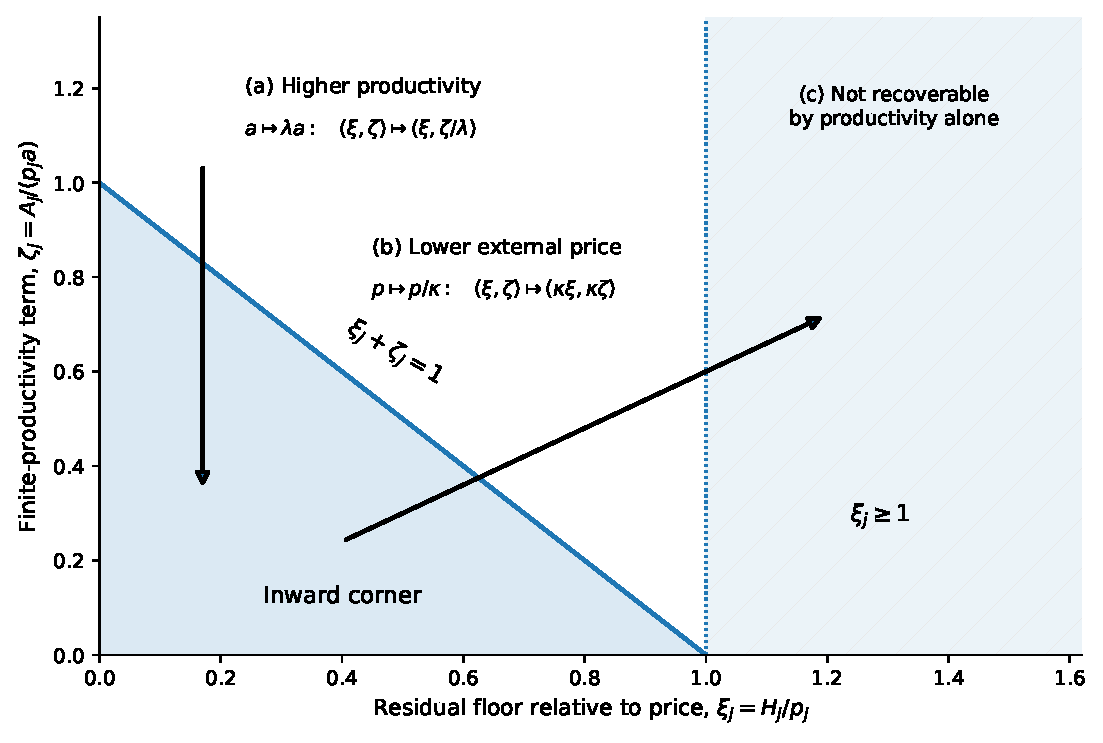
\includegraphics[width=.91\textwidth]{fig3.pdf}
\caption{Exact logarithmic phase diagram and comparative statics for one
external direction. The shaded triangle satisfies
$H_j/p_j+A_j/(p_ja)\leq1$; every external direction must satisfy this
condition for the all-inward corner to be optimal.
(a) Higher productivity reduces only $\zeta_j$, producing a downward
vertical move. (b) A price reduction to $p_j/\kappa$ multiplies both
coordinates by $\kappa$, producing a radial move away from the origin.
(c) In the hatched region $\xi_j\geq1$, no finite productivity restores
the corner. For $A_j>0$, $(1,0)$ is only a limiting point.
The arrows are schematic evaluations of the exact transformations;
no archived inputs are overlaid and no population frequency is estimated.}
\label{fig:phase}
\end{figure}

\subsection{Paired sensitivity design}
To distinguish deployment costs from access delays, use the normalized
family
\begin{equation}
 p_j=p_{j0}\left(f+\frac{1}{s_t}+\frac{0.2}{s_c}\right),\qquad
 r_j=r_{j0}m_r\exp(-0.1/s_t),\qquad a=a_0m_a.
 \label{eq:speed-map}
\end{equation}
Here $f>0$ is the residual price factor; $s_t,s_c>0$ index effective
material and information access speeds relative to $c$.
At instantaneous access, $p_j=p_{j0}f$ and $r_j=r_{j0}m_r$.
The coefficients $0.2$ and $0.1$ define scenarios, not calibrated physical
laws. Speed sweeps also remove the stipulated attenuation of remote
returns, so they are \emph{not} pure price experiments. The fixed-access
sweeps in $f$ isolate the price effect.

Faster-than-light access is only a counterfactual limiting case of this
map, not a physical mechanism established here. Instantaneous arrival
still leaves the positive deployment price $p_{j0}f$. Exactly zero
external prices are excluded: they can destroy compactness of the
feasible set and, with positive external computational returns and
unbounded increasing value, need not admit a finite optimizer.

The reference design contains 1,024 scrambled Sobol points in 14
dimensions, paired across every scenario. The exact library, generator
call and frozen inputs are specified in \cref{app:numerical}. Marginals
are log-uniform over the stated normalized ranges. The concave residual
benefits are
\begin{equation}
 E(x)=A_E(1-e^{-x/e}),\quad
 R(u)=A_R(1-e^{-u/r}),\quad
 I(v)=A_I(1-e^{-v/i}).
 \label{eq:benefit-family}
\end{equation}
The reference uses $(q,\epsilon_R,\epsilon_I,f)=(0.99,0.01,0.05,1)$
and $m_a=m_r=1$. Table~\ref{tab:scenarios} retains the full paired counts.

At instantaneous access, the reference has 219 inward corners; a
uniform $10\%$ price cut leaves 207. Only 364 reference inputs admit
a finite productivity threshold with the same residual slopes; the other
660 violate a residual-floor condition. Perfect experiential substitution
with zero residual weights yields 527 inward corners, while 497 still
prefer external computational capacity. Raising only local productivity
tenfold gives 314 inward corners; raising local and remote productivity
together gives 222. At $f=0.01$ and $f=10^{-4}$, the count is zero.
These are exact classifications of the archived inputs, not estimates of
civilizational prevalence.

Eight additional scrambles of 4,096 points each give instantaneous
inward fractions of \DesignLogMin--\DesignLogMax\% under the same
log-uniform marginals. Linear-uniform marginals over the same endpoints
give \DesignLinearMin--\DesignLinearMax\%. These 65,536 classifications
use the exact boundary. Their variation describes sensitivity to the
parameter-space measure, not observational uncertainty about the Galaxy.

\section{Future resources can reverse a present inward preference}
\label{sec:dynamic}

A one-horizon budget comparison omits one of the strongest reasons to expand: external industry can enlarge future resources. A minimal two-period construction makes this effect explicit while also allowing local investment to be productive. Let $B_1=10$, $z_1=B_1-p_1x$, and define
\begin{align}
 C_1(x)&=C_{01}+a_1\ln(1+z_1)+r_1x,\nonumber\\
 B_2(x)&=B_{20}+g_Lz_1+g_Xx,\label{eq:futurebudget}\\
 W(x)&=\ln[1+C_1(x)]+\beta V_2[B_2(x)],\quad 0\leq x\leq B_1/p_1.
 \label{eq:dynamic}
\end{align}
Here $B_1>0$, $B_{20},C_{01},C_{02}\geq0$, $a_1,a_2,p_1,p_2,r_1,r_2>0$, and $0\leq\beta\leq1$. The parameters $g_L,g_X\geq0$ convert current allocations to next-period resources. Both directions receive a future-production channel. All represented downstream benefits of first-period projects are captured through $B_2$; this is not a full persistent-capital or interstellar replication model.

The continuation value is the second-period pure-computation problem,
\begin{equation}
 V_2(B)=\max_{\substack{z_2,x_2\geq0\\z_2+p_2x_2\leq B}}\ln[1+C_{02}+a_2\ln(1+z_2)+r_2x_2].
 \label{eq:continuation}
\end{equation}
For $r_2>0$,
\begin{equation}
 z_2^*(B)=\min\{B,\max(a_2p_2/r_2-1,0)\},\qquad
 x_2^*(B)=\frac{B-z_2^*(B)}{p_2}.
 \label{eq:stage2}
\end{equation}
Its marginal value $V_2'(B)$ is the current best computational marginal return divided by $1+C_2^*(B)$: $a_2/(1+B)$ on the all-local branch, or $r_2/p_2$ on the mixed/external branch. The expressions agree at the switching budget. $V_2$ is increasing and concave.

\begin{proposition}[A future-adjusted inward condition]
\label{prop:dynamic}
For \cref{eq:dynamic,eq:continuation}, the all-inward first-period allocation is optimal if and only if
\begin{equation}
 \frac{r_1-p_1a_1/(1+B_1)}{1+C_{01}+a_1\ln(1+B_1)}
 +\beta V_2'(B_{20}+g_LB_1)(g_X-p_1g_L)\leq0.
 \label{eq:dynamiccriterion}
\end{equation}
\end{proposition}
\begin{proof}
The first term in $W$ is concave in $x$, and composition of concave $V_2$ with affine $B_2(x)$ is concave. For a differentiable concave function on an interval, the left endpoint is a global maximizer exactly when its right derivative is non-positive. Differentiating \cref{eq:dynamic} at zero gives \cref{eq:dynamiccriterion}.
\end{proof}

The first term is the original within-period comparison. The second values the \emph{difference} between external and local production of future resources. Counting $g_X$ while setting $g_L$ to zero without justification would bias the test against inward development; omitting $g_X$ would bias it in favour. This extension is a structural check, not a calibrated decision rule for actual civilizations.

For $p_1=p_2=r_1=r_2=1$, $a_1=a_2=100$, $C_{01}=C_{02}=B_{20}=1$, $g_L=0.2$, and $\beta=0.9$, present-only investment is all inward. The future-adjusted corner changes at $g_X=\DynamicThreshold$. At $g_X=0.2$ both periods remain all inward. At $g_X=2$, optimal first-period outward investment is $x=\DynamicOutward$, leaving $z_1=6.2441$ locally and producing $B_2=9.7607$. All second-period investment is still local. Thus the optimal path can include \emph{external investment undertaken to finance later inward activity}. This differs from claiming that external expansion is never useful. \Cref{fig:dynamic} gives the full 201-setting construction.

\begin{figure}[tbp]
\centering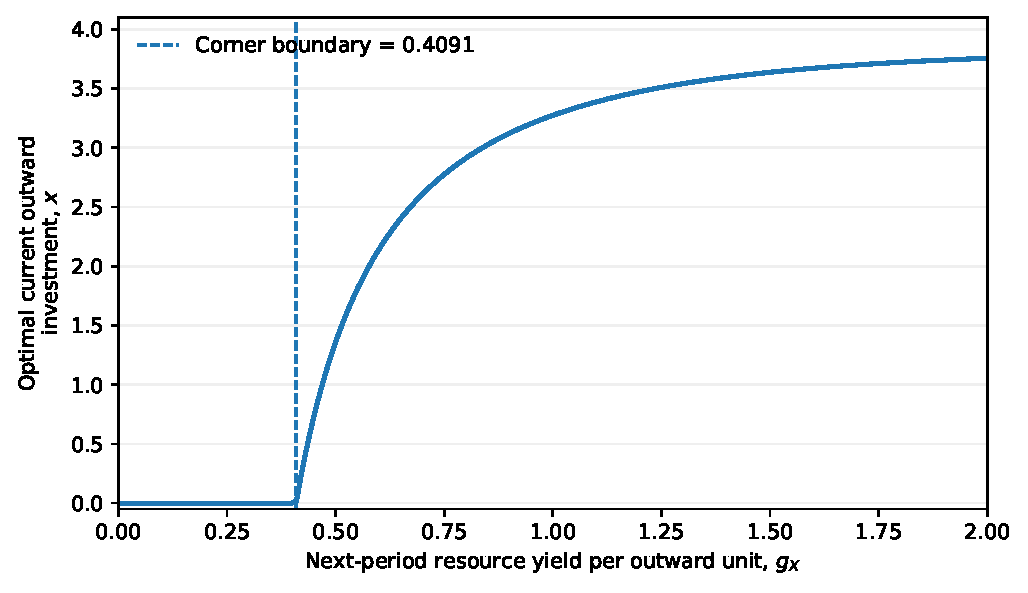
\includegraphics[width=.95\textwidth]{fig4.pdf}
\caption{Two-period resource feedback. Local investment generates future resources at $g_L=0.2$ per unit. Increasing the external yield $g_X$ eventually overturns the all-inward present-only optimum. Parameters are normalized; the transition is an exact derivative boundary checked against a separate three-variable numerical optimization.}
\label{fig:dynamic}
\end{figure}

The converse reversal is also possible. Keep
$B_1=10$, $p_1=p_2=r_1=r_2=1$ and $\beta=0.9$, but set
$a_1=5$, $a_2=100$, $C_{01}=C_{02}=1$, $B_{20}=0$,
$g_L=0.1$ and $g_X=0$. The static term in
\cref{eq:dynamiccriterion} is $\ReverseStaticTerm$, and the
present-only optimum is $x=\ReverseStaticX$. The continuation term is
$\ReverseFutureTerm$, making the total $\ReverseTotalTerm$.
Concavity therefore makes $x=\ReverseDynamicX$ the two-period optimum.
Local investment, rather than external investment, produces the more
valuable continuation budget in this example. Supplementary Material
section~S3 reports scalar and joint-optimization checks of both cases.

Thus static inwardness is neither sufficient nor necessary for dynamic
inwardness: the $g_X=2$ example disproves sufficiency, and the converse
example disproves necessity. For these two examples, all second-period
investment is local at the dynamic optimum. The same logical failures
can be embedded in an infinite horizon by appending a summable discounted
continuation whose budgets and returns are independent of the first
two periods' allocations and whose subsequent optima are all inward. Such a continuation adds a constant
to the current comparison and leaves its optimizer unchanged. This
establishes the absence of a universal implication, not an
infinite-horizon policy theorem for persistent capital or resource
accumulation. Proposition~\ref{prop:persistence} remains a
characterization of repeated static choices; section~7.2 states the
corresponding limitation.

\section{From an inward civilization to a quiet galaxy}
\label{sec:population}

\subsection{Initiation, survival, and arrival are not the same event}

A civilization contains heterogeneous agents. A scalar objective in \cref{eq:utility} is a representation of a specified decision process, not proof that every inhabitant shares its preferences. Recursive virtual population growth is especially relevant to this distinction. More virtual agents increase the potential expansionist population only when they possess physical agency, obtain access to actuators, or can create outward-capable descendants. Reliable containment might reduce that exposure, but it is not guaranteed by virtuality.

Let $a_i(t)$ be outward-capable autonomous nodes and $\lambda_i(t)$ their initiation rate per node-time. Under an independent Poisson approximation, the expected number of successful fronts from one civilization is
\begin{equation}
 \mu=\sum_i\int\lambda_i(t)a_i(t)[1-q_{R,i}(t)]\dd t.
 \label{eq:mu}
\end{equation}
For a Galton--Watson process with offspring generating function $G_R$, the extinction probability is the smallest solution $q_R=G_R(q_R)$; for Poisson offspring with mean $\Rogue$, $q_R=\exp[\Rogue(q_R-1)]$ \citep{Harris1963}. Standard non-degenerate processes become extinct almost surely when $\Rogue\leq1$. Survival for $\Rogue>1$ is not equivalent to occupying the Galaxy or reaching Earth.

For a fixed independent list of civilizations with Poisson front means $\mu_i$,
\begin{equation}
 P_0^{\rm fixed}=\exp\left(-\sum_i\mu_i\right).
 \label{eq:fixed}
\end{equation}
If civilization origins instead form a Poisson process with intensity measure $\nu(\dd z)$, independently marked by their front distributions, then
\begin{equation}
 P_0^{\rm origins}=\exp\left[-\int(1-e^{-\mu(z)})\nu(\dd z)\right].
 \label{eq:origins}
\end{equation}
This follows from the Poisson generating functional \citep{LastPenrose2017}. The fronts are clustered within their parent civilizations; replacing $1-e^{-\mu}$ by $\mu$ is only a small-$\mu$ approximation. For $N=\bar N=2$ and $\mu=2$, the fixed-population and random-origin probabilities are approximately $0.0183$ and $0.1774$, respectively. Separate 250,000-realization simulations check these formulas.

To explain a null observation in a specified region by time $T$, replace $\mu(z)$ by the mean number $\mu_A(z,T)$ of front initiations that both survive and arrive under an explicit propagation model. Faster access can enlarge this arrival exposure even if typical investment remains inward. The allocation simulations do not calculate $\mu_A$ or a probability of galactic silence. Subcritical lineages can also produce finite local artefacts before extinction. Frequency among origins is therefore not frequency among occupied systems.

\subsection{Visibility and non-identifiability}

Settlement, industry, and observation indices do not determine power, spectrum, geometry, or duty cycle. A compact computational civilization may use substantial stellar power, while a wide probe network may be faint. The Dyson--Kardashev energy-processing tradition addresses observability but is not a direct scale of welfare or settlement demand \citep{Dyson1960,Kardashev1964}. Galaxy-scale infrared searches require a physical emission model and selection function \citep{Wright2014a,Wright2014b}.

For mutually exclusive source classes with approximately independent Poisson detections,
\begin{equation}
 \Lambda_j(T)=\int_0^T R_{\rm civ}(t_e)S_j(T-t_e\mid t_e)\pi_j(T,t_e)\dd t_e,
 \qquad P(0)=e^{-\sum_j\Lambda_j}.
 \label{eq:observations}
\end{equation}
Here $S_j$ is a source-state probability and $\pi_j$ a selection probability. Overlapping settlement, industry, and probe attributes require a union-detection probability rather than a sum that counts an object twice. Even in a stationary single-class reduction, a null result constrains the product $R_{\rm civ}\tau\bar\pi$, not its factors separately. Multiplying the emergence rate by a factor and dividing detectability by the same factor leaves the likelihood unchanged when the parameters remain admissible. Non-detection alone cannot identify inward transition.

Recent observations illustrate this distinction. Project Hephaistos II identified seven follow-up candidates from approximately five million sources \citep{Suazo2024}. The cited 2026 JWST study attributes the excesses of two candidates to background galaxies \citep{Zackrisson2026}. A separate preprint tests warm technological components in 129 nearby galaxies without a preferred positive component \citep{Curtis2026}. These reports constrain the searched emission models; they do not establish virtual civilizations, universal low detectability, or the feasibility of local recursive growth. Solar-System artefact searches address another relevant class \citep{Freitas1983,HaqqMisraKopparapu2012}.

The weaker settlement-composition branch suggests comparing resident infrastructure with automated industrial and information artefacts after correcting their selection functions. The wholly inward branch need not produce those distant artefacts. To discriminate the mechanism, a future study would need independently constrained resource budgets, support capacity, substitution behaviour, or a population of signatures for which intensive activity and outward acquisition can be estimated separately. 

\section{Verification, limitations, and interpretation}
\label{sec:verification}
\subsection{What is verified}
Separate AI-assisted implementations reconstruct the equations without
importing the generating model. The exact logarithmic test reproduces
all 14,336 archived corner classifications; 11,002 tests check both sides
of finite positive productivity thresholds. The stored optimized shares
also pass objective, feasibility and concavity-gap checks. Scalar and
joint optimizations check the curvature examples, production alternative,
pure-computation budget solution and two-period extension; direct
accounting checks the workload examples, including the memory failure
beyond the stated horizon. Complete proofs establish the mathematical
claims; these numerical tests check implementations and examples, not
extraterrestrial premises. Supplementary Material sections~S1--S3 provide
certificate details, executable commands, numerical outputs and the
seed-versus-\texttt{rng} comparison. Frozen inputs, environment versions
and integrity manifests accompany the source.

\subsection{Limitations that change the conclusion}
\label{sec:limitations}
\paragraph{Physical support and recursive interpretation.}
The workload frontier is a homogeneous service model, not an engineered
architecture or a test of consciousness. Efficiency or fidelity may
plateau, stored state may dominate memory, and digital population growth
may restore scarcity. Per-agent resources increase only if useful
computational growth outpaces agent growth. The fixed-budget joint witness
chooses rather than derives its productivity path. No engineering model
here establishes indefinite growth of every effective support capacity.
Recursion is neither necessary nor sufficient for inward allocation.

\paragraph{Preferences, production and mathematical scope.}
The objective represents a specified decision process, not a shared
utility function of every inhabitant. Divisible investment, positive
prices, differentiability and concavity are substantive restrictions.
The local logarithm and external production functions are not empirically
identified; \cref{lem:production} separates corner robustness from
interior-allocation sensitivity. The value-curvature parameter also
changes the conclusion, as \cref{prop:curvature} shows. Small residual
utility weights do not certify physical safety or remove the value of
geographically independent backups. Fixed project sizes, start-up
thresholds and increasing returns can invalidate a local test. For example,
\begin{equation}
 U(x)=\ln\{1+2\ln(2-x)+0.1x\}+3x^2,\qquad 0\leq x\leq1,
 \label{eq:nonconcave}
\end{equation}
with $z=1-x$, has $U'(0)\simeq-0.3772$, yet
$U(1)\simeq3.0953>U(0)\simeq0.8697$. This violates the concavity
assumption rather than \cref{prop:corner}. Under added hard constraints,
necessity of the corner inequalities additionally requires the proposed
small budget-transfer directions to remain feasible.

\paragraph{Persistence and future opportunities.}
Proposition~\ref{prop:persistence} characterizes a sequence of static
optima, not an infinite-horizon policy. Its conditions are neither
necessary nor sufficient, in general, for an all-inward optimal policy
in a dynamic model: section~\ref{sec:dynamic} gives both reversals in two periods and
explains their extension when the later continuation is independent.
A substantive infinite-horizon criterion would require specified state
dynamics, feasible policies, and a well-defined discounted or long-run
objective. With logarithmic value, fixed positive residual slopes and bounded prices
exclude an all-inward path when budgets become unbounded. Residual decay
or sufficiently rising relative prices must satisfy the exact productivity
condition as well; simply observing that $S_j(t)\to0$ is insufficient.
The two-period model includes both local and external future resource
production, but not a full ecology of accumulated capital, strategic
competition, irreversible settlement, survival or real options.

\paragraph{Access and physical assumptions.}
The access-cost map is a sensitivity family, not a propulsion model.
Proposed warp geometries do not establish operational faster-than-light
travel \citep{Alcubierre1994}; energy-condition and causality objections
remain relevant \citep{Everett1996,Santiago2022}. The counterfactual
limiting cases assume consistent scheduling without usable travel into
one's own past. A rapid material courier may also carry information.
Faster access can increase both external opportunities and arrival
exposure, not merely reduce travel time.

\paragraph{Inference about populations.}
The synthetic design is not an astronomical prior. Neither its counts nor
variation across scrambles estimates the prevalence of inward civilizations.
Allocation does not identify power use, spectra, duty cycles, autonomous
expansionist exposure or arrival probabilities. Survey nulls are therefore
not selective confirmation of \CITH. Empirical application would require
independent evidence for relevant resource and preference parameters,
a propagation model and comparative observational likelihoods.

\section{Conclusion}
The relevant possibility is a growing civilization, not necessarily a
satiated or inactive one. Internal computational uses, including recursively
generated virtual worlds, can compete successfully with additional external
projects. The resource frontier and the common-budget model make the two
requirements distinct: the chosen workload must remain physically
supportable, and inward investment must remain preferable at the relevant
opportunity costs.

Continued internal growth with no additional external investment is
therefore conditional on a path, not established by a favourable corner
at one budget. Under logarithmic computational value, budgets tending to
infinity, fixed positive residual external slopes and bounded relative
prices are incompatible with persistent all-inward allocation, irrespective
of productivity. Persistence requires the price-to-residual-slope ratio to
exceed $(1+B)\ln(1+B)$ wherever a residual slope is positive, together
with the exact productivity threshold and continuing local feasibility.
The curvature extension further shows that the finite residual floor is
specific to logarithmic value: slower marginal-value decay permits an
eventual productivity threshold at fixed budgets and prices, whereas
faster decay makes sufficiently high productivity incompatible with
inwardness when residual slopes are positive.

Concave external alternatives preserve the corner comparison when initial
returns are unchanged, but alter mixed allocations. Cheap external access
and future resource production supply additional reasons to expand.
These boundaries define a quantitatively specified alternative to
inferring inevitable expansion from capability alone.
They do not establish its prevalence, indefinite engineering realization,
or a population-level explanation of galactic silence.

\section*{Declarations}

\paragraph{Data and code availability.} All model data are normalized synthetic inputs. The accompanying source-and-replication package contains the frozen allocation inputs and optimized solutions, separate equation-level audit code, workload and budget checks, full proofs, new curvature and pathwise tests, figure arrays, environment records, and SHA-256 manifests. Reproduction commands and the exact Sobol generator call are given in \cref{app:numerical} and the Supplementary Material. No public repository DOI is asserted; these materials should accompany submission.

\paragraph{Author information.} Hyeonjun Joo is an independent researcher in the Republic of Korea. Correspondence: \href{mailto:jonejoo0805@gmail.com}{jonejoo0805@gmail.com}.

\paragraph{Financial support and competing interests.} The author reports no specific funding and no competing interests.

\paragraph{Author contributions.} Hyeonjun Joo: Conceptualization; Methodology; Formal analysis; Investigation; Visualization; Writing; Project administration. The author is responsible for approving the scientific interpretation and final manuscript.

\paragraph{Use of artificial-intelligence tools.} OpenAI ChatGPT assisted mathematical model development, code generation, computational checks, literature checking, language revision, and LaTeX preparation, including the work dated 12 October 2026. Both the generating and checking implementations were AI-assisted. Separate implementations do not constitute independent human peer review. All plotted values come from archived calculations. The human author retains responsibility for the scientific claims, references, numerical results, final wording, and submission decision. No AI system is an author.

\paragraph{Ethics.} No human participants, animals, personal research data, or identifiable-person observational data were studied.

\appendix
\section{Numerical specification and paired results}
\label{app:numerical}

The canonical unit points and transformed parameters are the arrays
\texttt{sobol\_vectors} and \texttt{parameters} in
\texttt{data/allocation/design.npz}. The generating environment records
Python~3.13.5, NumPy~2.3.5 and SciPy~1.17.0. The exact call is
\begin{verbatim}
from scipy.stats import qmc
u = qmc.Sobol(d=14, scramble=True,
              seed=20260905).random_base2(m=10)
\end{verbatim}
The default \texttt{bits=None} resolves to 30 bits; optimization is
\texttt{None}. No points are skipped or thinned. For the ordered endpoint
vectors in \cref{tab:ranges}, the transformation is
\begin{verbatim}
lo = np.log(lower_endpoints)
hi = np.log(upper_endpoints)
parameters = np.exp(lo + u * (hi - lo))
\end{verbatim}
Every scenario uses the same transformed rows.

Re-execution in SciPy~1.17.0 reproduces the archived unit points bit for
bit. Floating-point exponentiation changes some transformed entries by
at most a relative $2.22\times10^{-16}$ in the present environment;
all classifications agree. Evaluation of the frozen arrays reproduces
219 instantaneous-reference inward corners and 527 under perfect
substitution with zero residual weights, as well as all other counts
in \cref{tab:scenarios}.

With \texttt{seed=20260905}, the archived unit points are reproduced
bit for bit under SciPy~1.17.0 and 1.18.1;
\texttt{rng=20260905} yields a different scramble, with 208
instantaneous and 530 perfect-substitution inward corners.
The frozen arrays, not the seed alone, define the reference experiment.
Supplementary Material section~S2 records the generator specification
and file checksums.

The parameter order is $(B,C_0,a,r_n,r_h,A_E,A_R,A_I,e,r,i,p_{n0},p_{h0},p_{m0})$. All base marginal ranges are log-uniform in the reference experiment. Values of $e,r,i$ in this appendix are return scales, not energy, radius, or individual identifiers.

\begin{table}[htbp]
\centering
\caption{Normalized ranges in the 14-dimensional reference design.}
\label{tab:ranges}
\begin{tabular}{@{}lll@{}}
\toprule
Quantity & Range & Meaning\\
\midrule
$B$ & $1$--$100$ & common investment budget\\
$C_0$ & $0.1$--$10$ & existing useful computational service\\
$a$ & $1$--$1000$ & intensive computational coefficient\\
$r_n,r_h$ & $0.1$--$10$ & external computational returns\\
$A_E,A_R,A_I$ & $0.1$--$10$ & benefit amplitudes\\
$e,r$ & $1$--$30$ & experiential and resilience scales\\
$i$ & $1$--$100$ & information scale\\
$p_{n0}$ & $1$--$10$ & resident unit price\\
$p_{h0}$ & $0.1$--$3$ & industry-only unit price\\
$p_{m0}$ & $0.01$--$0.3$ & observation-only unit price\\
\bottomrule
\end{tabular}
\end{table}

The sublight scenario has $(s_t,s_c)=(0.01,1)$, the communication-only variant $(0.01,\infty)$, the light-speed case $(1,1)$, and combined faster-access cases $(10,10)$, $(1000,1000)$, and $(\infty,\infty)$. The no-substitution variant sets $q=0$. Large residual values set $\epsilon_R=\epsilon_I=1$, either retaining $q=0.99$ or additionally setting $q=0$. The two tenfold productivity variants set $(m_a,m_r)=(10,1)$ and $(10,10)$. The perfect-substitution variant sets $(q,\epsilon_R,\epsilon_I)=(1,0,0)$. Reduced-price variants set $f=0.01$ or $10^{-4}$ with instantaneous access; other parameters remain at reference settings. A material-speed variable is not allowed to make numerical prices exactly zero.

\begin{table}[htbp]
\centering\small
\caption{All-inward inputs out of 1,024, with a conditional price-robustness check. The last column applies a uniform 10\% price reduction to each listed scenario while retaining its other settings. It is computed from the exact boundary, not from a new behavioral assumption or an observational sample.}
\label{tab:scenarios}
\begin{tabularx}{\textwidth}{@{}Xrr@{}}
\toprule
Scenario & All inward & Still inward after 10\% price cut \\
\midrule
Sublight material travel & 929 & 923 \\
Fast communication only & 929 & 923 \\
Light-speed limit & 326 & 313 \\
Travel and communication at 10c & 234 & 219 \\
Travel and communication at 1000c & 219 & 207 \\
Instantaneous reference & 219 & 207 \\
No experiential substitution & 146 & 135 \\
Large residual values & 14 & 14 \\
No substitution + large residuals & 11 & 10 \\
Local productivity $\times10$ & 314 & 296 \\
Local and remote productivity $\times10$ & 222 & 211 \\
Perfect substitution; no residual values & 527 & 505 \\
Outward price floor $\times0.01$ & 0 & 0 \\
Outward price floor $\times0.0001$ & 0 & 0 \\
\bottomrule
\end{tabularx}

\end{table}

Corner classification uses the exact inequalities, not optimizer-selected shares. The stored optimal shares are checked separately using the objective and concavity certificates described in Supplementary Material section~S1. Small platform-dependent changes in transformed parameters or nearly tied optimized shares do not change any archived corner classification in the checks reported here.

For design-measure sensitivity, Sobol seeds 20260911 through 20260918 each generate $2^{12}$ points. Both log-uniform and linear-uniform transformations use the same bounds in \cref{tab:ranges}. Repeated scrambles assess numerical integration stability under a selected measure. They do not supply a prior justified by extraterrestrial observations.

